%!TEX root = ../main.tex
%%%%%%%%%%%%%%%%%%%%%%%%%%%%%%%%%%
% Links:
%
% Difficulty: Companies: 
%%%%%%%%%%%%%%%%%%%%%%%%%%%%%%%%%%


%\begin{figure} \centering 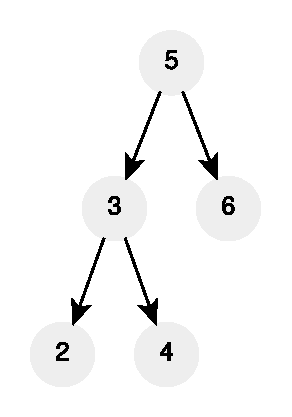
\includegraphics[width=\textwidth]{sources/count_bits/images/example1}
%   \caption[Sample short cpation]{Sample Caption}. \label{fig:count_bits:example1} \end{figure}

\chapter{Count the bits}
\label{ch:count_bits}

\section*{introduction}
Computers use binary numeral system to store data and perform computations. In this system a bit
is the smallest unit of data and can only have value $0$ or $1$. By using several bits we are able to encode information such as documents,  music, books, maps, bitcoins, etc. Ultimately the binary numeral system is just a way of representing numbers and it is not really different from the decimal system we use everyday.
A binary number is made up of one or more bits, the same way a decimal number is made up of several $0-9$ digits. For instance, the binary number $111111001000011111010110_2$ correspond to the decimal number $16549846$.

In programming, binary numbers are often used as bitsets as a more efficient and memory cheat substitute to arrays of booleans; such use case is so common that in the \CC STL we even have a dedicated class: \href{https://en.cppreference.com/w/cpp/utility/bitset}{\inline{std::bitset}}. However a simple \inline{int} can be used as a bitset and in this chapter we will calculate some statistics on the number of bits that are set to \inline{true} in a bitset (pretty much equivalently to what the function \href{https://en.cppreference.com/w/cpp/numeric/popcount}{\inline{std::popcount(T x)}} does) for a range of numbers.

This problem is aimed at testing our basic bit manipulation skills and all we need to get a woking solution is knowing how to use some basic bit logic operations and functions like \textit{shift} and  \textit{AND}. Besides this basic solution we will also have a look at two more sophisticated and efficient solutions: the former based on DP and the second based on a property of powers of two. 



\section{Problem statement}
\begin{exercise}
\label{example:count_bits:exercice1}
Given a non negative integer number $n$ return an array $B$ of size $n+1$ where $B_i$ contains the
number of bits set in the number $i$.
	%example1
	\begin{example}
		\label{example:count_bits:example1}
		\hfill \\
		Given $n = 5$ the function returns $B = \{0,1,1,2,1,2,2\}$	
	\end{example}

\end{exercise}

\section{Clarification Questions}

\begin{QandA}
	\item \begin{questionitem} \begin{question} Can we assume $n$ is always positive?  \end{question} 	 
    \begin{answered}
		\textit{Yes, you do not have to perform any input validation.}
	\end{answered} \end{questionitem}
	
\end{QandA}

\section{Discussion}
\label{count_bits:sec:discussion}


\subsection{Na\"ive approach solution}
\label{count_bits:sec:bruteforce}
This is an easy problem. All we have to do is to brute-force our solution by counting
the number of bits set for each and every number from $0$ to $n+1$. Each number has a fixed size
which on most the common modern C++ implementation is $32$-bit (\inline{sizeof(int)}) and therefore
we can come up with a $\Theta(32n)$ solution. Counting the bits of a given integer can even be done
with
\href{https://gcc.gnu.org/onlinedocs/gcc-4.9.2/gcc/X86-Built-in-Functions.html}{compiler intrinsics}
as \inline{__builtin_popcount} which can map directly when supported by the hardware to fast
machine instructions or by using some simple bit manipulation trickery. From C++20 we can also use
the \inline{std::popcount} function, together with a several other  bit related functions (in the
header \inline{<bit>}). Listing \ref{list:count_bits:bruteforce} shows an implementation of this
idea where we use our own version of the bit counting function \inline{my_pop_count} for the sake of
showing how this can be implemented. Function \inline{my_pop_count} works by repeatedly inspecting
the least significant bit of of the input number to check if it is set or not and after that it
shifts it to the right by one position so that the next time another bit is inspected.
\lstinputlisting[language=c++, caption={Bruteforce solution where we manually count the number of bits for each number.},label=list:count_bits:bruteforce]{sources/count_bits/count_bits_solution1.cpp}

\subsection{DP solution}
\label{count_bits:sec:dp}
This problem can be solved more elegantly using dynamic programming. This approach also does
not incur a factor $32$ penalty for the count of the bits of a number.

The idea is that the number of bits set for a given number is equal to the number of bits set in the
same number shifted one position to the right (removing the last bit), which is always smaller than
the number we started with, plus one if the removed bit was $1$.

For instance consider $x=2730_{10} = 101010101010_2$. The least significant bit of $x$ is $0$
therefore its number of bits set is equal to the number of bits set of $y=1365_{10} = 10101010101_2$
(last bit removed). For the same reasons the number of bits set in $y$ is one (because the last bit
is $1$) plus the number of bits set in $y=682_{10} = 1010101010_2$(last bit removed). We can follow
this line of reasoning until we reach $0$ which clearly has zero bits set.

Given that every time we remove a bit we are solving a problem for a smaller number and because the
solution for a number $x$ can be required to count the bits of many numbers $n>x$, we can adopt
DP(see Appendix \ref{sect:appendix:DP}) (it exposes optimal substructures as well as overlapping subproblems). In a
DP solution we will use  a DP table $B$, which we initially fill only for the number $0$. We will
then follow a bottom-up approach where we start solving problems for $x=1,2,\ldots,n$. When we
reach a given number $y$ we have already solved and stored into $B$ the answers for every number less
than $y$, therefore we can count the number of bits in $y$.
Moreover because the answers for all of
these numbers smaller than $y$ are stored in $B$ we do not need to recompute them. 

Listing \ref{list:count_bits:DP} shows an implementation of this approach. You can find a shorter (three
lines) more compact ( although possibly unreadable) but equivalent version of the same idea in
Listing \ref{list:count_bits:DP_short}.

\lstinputlisting[language=c++, caption={DP solution where we calculate the bits for a given number from the its last bit and the answer of the number resulting from removing that last bit.},label=list:count_bits:DP]{sources/count_bits/count_bits_solution2.cpp}

\lstinputlisting[language=c++, caption={ Shorter version of Listing \ref{list:count_bits:DP}.},label=list:count_bits:DP_short]{sources/count_bits/count_bits_solution3.cpp}

\subsection{Another efficient approach}
\label{count_bits:sec:pattern}
There is another way of solving this problem which is quite different from the DP approach we
discussed above. Let's start by noting that any power of $2$ always has one and only one bit set.
For instance $2^2$ has the bit at index $2$ set and the rest of the bits not set. The same applies
for any other power of two $2^k$ where only the bit at index $k$ is set. All the numbers from $2^k$
to $2^{k+1}-1$ can be obtained by concatenating a $1$ (the bit at index $k$) with all the binary
representations of the numbers from $0$ to $2^k-1$ (all the numbers smaller than $2^k$).

For instance let's take $k=4$ as an example. All the numbers from $2^4 = 16$ to $2^5-1 = 31$ can be
obtained as shown below:
\begin{itemize}
	\item $16 = 16+0 = 10000_2+ 0_2$
	\item $17 = 16+1 = 10000_2+ 1_2$
	\item $18 = 16+2 = 10000_2+ 10_2$
	\item $19 = 16+3 = 10000_2+ 11_2$
	\item $20 = 16+4 = 10000_2+ 100_2$
	\item $21 = 16+5 = 10000_2+ 101_2$
	\item $22 = 16+6 = 10000_2+ 110_2$
	\item $23 = 16+7 = 10000_2+ 111_2$
	\item $24 = 16+8 = 10000_2+ 1000_2$
	\item $25 = 16+9 = 10000_2+ 1001_2$
	\item $\ldots$
	\item $31 = 16+15 = 10000_2+ 1111_2$
\end{itemize}
As you can see the answer for all the numbers from $16$ to $31$ can be calculated by adding one to
the answer of all the rest of the numbers we have already calculated (the numbers from $0$ to $15$).
The same applies for smaller $k$. For $k=2$ we have:
\begin{itemize}
	\item $4 = 4+0 = 100_2+ 0_2$
	\item $5 = 4+1 = 100_2+ 1_2$
	\item $6 = 4+2 = 100_2+ 10_2$
	\item $7 = 4+3 = 100_2+ 11_2$
\end{itemize}
We can use this idea to build a fast and efficient solution which is shown in Listing \ref{list:count_bits:powers}.
The answers are calculated incrementally starting with the integers $0$, $1$ and $2$ which have $0$,$1$ and
$1$ bits set, respectively.
Then we can calculate the answer for $2$ and $3$ (from $2^2$ to $2^3-1$)
by adding $1$ to the answers for $0$ and $1$.
For the numbers from $4$ to $7$ ($2^2$ to $2^3-1$) we
add $1$ to the answers to $0$, $1$ and $2$ and $3$, respectively.
For the numbers from $8$ to $15$ ($2^3$ to
$2^4-1$) we add $1$ to the answers for $0, 1, \ldots,7$.
We keep doing this, adding $1$ to all the
numbers from $0$ to $2^k-1$ in order to calculate the answer for all the numbers from $2^k$ to
$2^{k+1}-1$, until we reach $n+1$.
The complexity of this approach is $\Theta(n)$ and also in this
case we do not pay the constant factor associated with a brute-force count of the bits in an
integer.
\lstinputlisting[language=c++, caption={Alternative efficient solution where the number of bits set in a integer $k$ is found by using the number of bits set for a smaller integer: $k-(2^{\lfloor log_2{k \rfloor}})$ (see Equation \ref{eq:count_bits:dpformula_powers}).},label=list:count_bits:powers]{sources/count_bits/count_bits_solution4.cpp}

Note that the same approach can be easily adopted to obtain a top-down implementation where we memoize and reuse the answer to how many bits a given integer has set.
We leave this  as an exercise for the reader \footnote{The recurrent relation to the number of bits set in $k$ is as shown in Equation \ref{eq:count_bits:dpformula_powers} where $B(x)$ is a function returning the number of bits set in the binary representation of the integer $x$:
\begin{equation}
	\begin{cases}
		B(0) = 0 \\
		B(1) = 1 \\
		G(k) =  1 + G(k-(2^{\lfloor log_2{k \rfloor}})) 	 \end{cases}
	\label{eq:count_bits:dpformula_powers}
\end{equation}
}.